It is worthwhile to first discuss the quality of the model used, and its relationship to reality.
\Cref{fig:eeg} shows several types of behavior one can expect on an EEG trace.
\begin{figure}[ht]
  \centering
  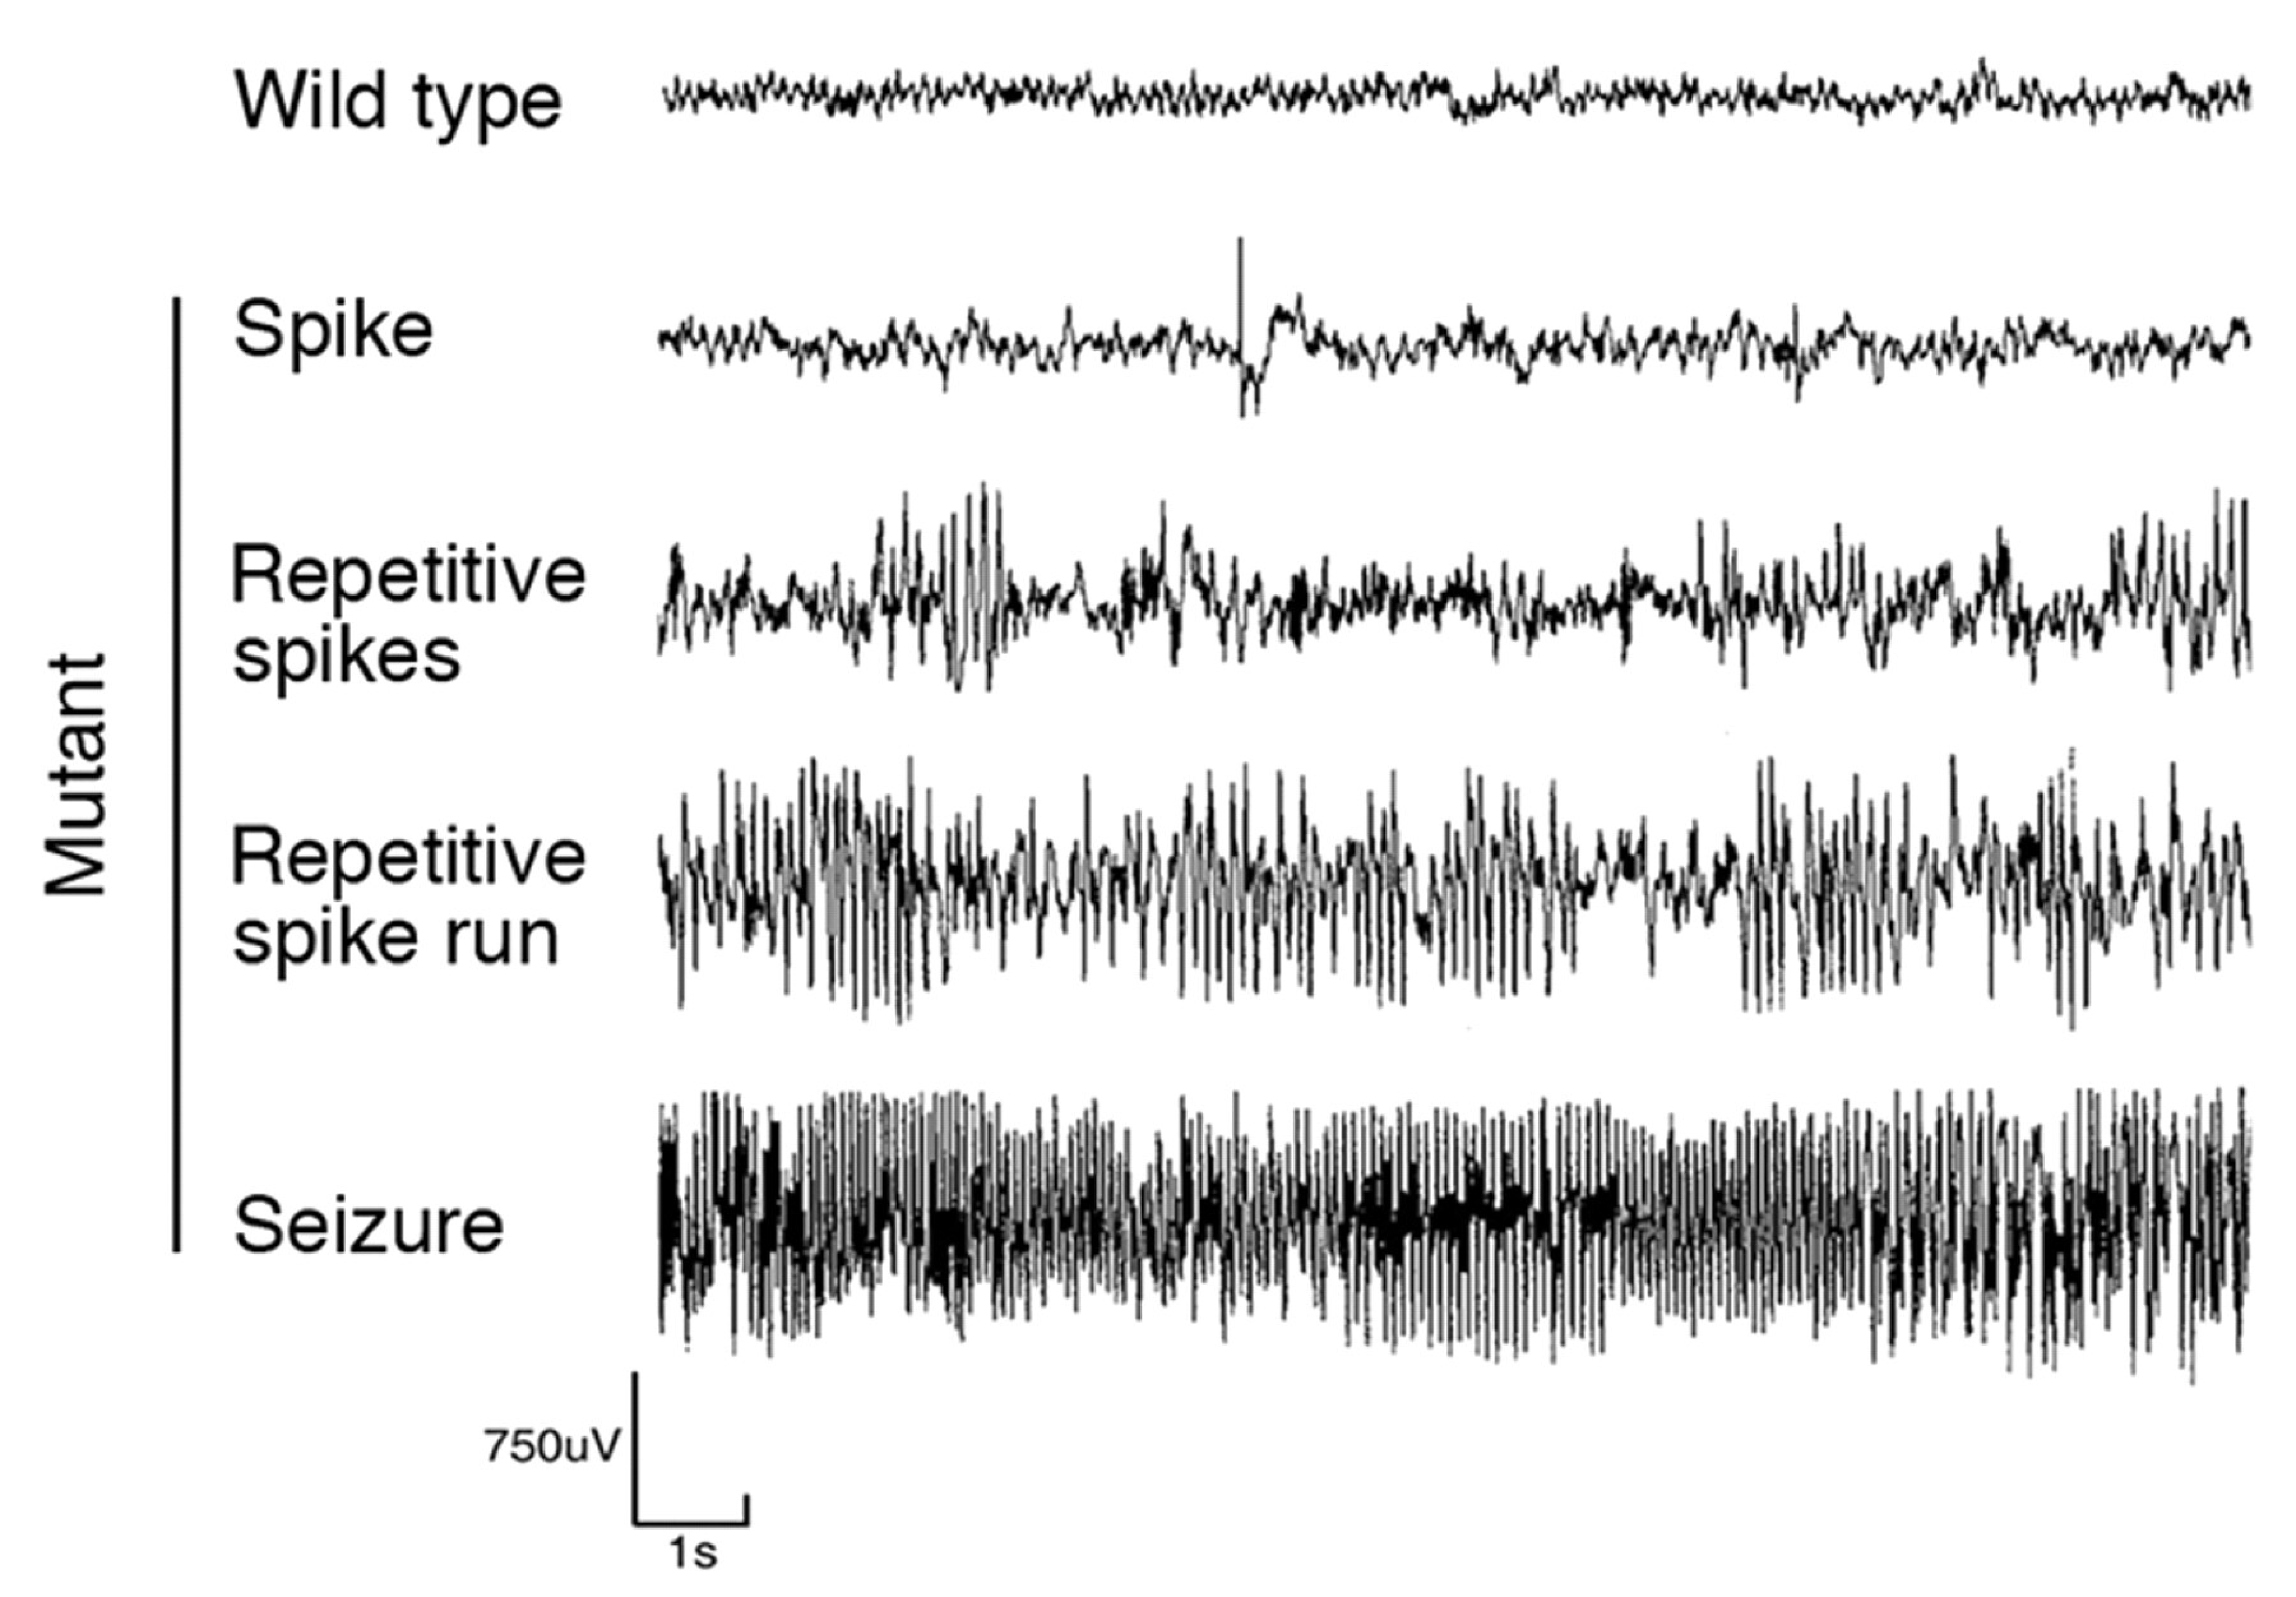
\includegraphics[width=0.5\textwidth]{figure/eeg.pdf}
  \caption[Typical EEG trace]{A typical EEG trace.
    The first row (``Wild type'') shows a normal awake adult mouse EEG trace.
    The other four rows (``Mutant'') show typical abnormal/epileptiform activity.
    Taken from \cite{Ljungberg2009}.
  }
  \label{fig:eeg}
\end{figure}
Healthy brain behavior presents as low-amplitude oscillations on an EEG, as the asynchrony leads the firings of individual neurons to cancel each other out.
Seizures and seizure-like activity present as higher-amplitude oscillations, as the synchrony decreases the variance between neurons, making the mean closer to the behavior of each neuron.
One of the main challenges of simulating seizures is that only trained experts can truly identify seizures; as yet, there is no mathematical technique for identifying seizures \cite{Kandel2013}.

\begin{figure*}[ht]
  \centering
  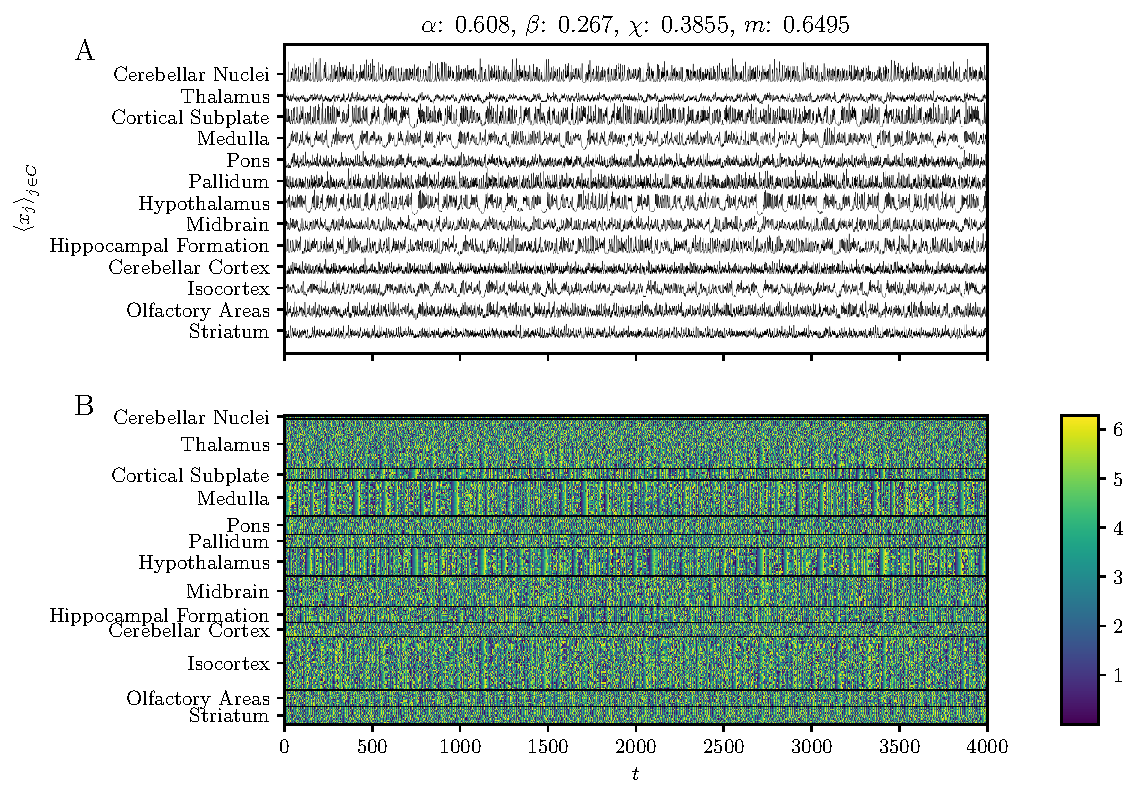
\includegraphics[width=\textwidth]{figure/0_608-0_267_200dpi.pdf}
  \caption[Typical simulation]{A typical run of the Hindmarsh-Rose simulation.
    A. The mean membrane potential within each cortex.
    B. The phase $\phase$ of the entire timeseries for a simulation of the Hindmarsh-Rose network.
  }
  \label{fig:608_267}
\end{figure*}

The highly chimeric portion of the landscape appears to be mostly below the $\beta = \alpha$ line.

However, one can indicate whether a model resembles epileptiform activity on a qualitative level.
\Cref{fig:608_267} shows the results of a simulation of the Hindmarsh-Rose network for $\pqty{\hra, \hrb} = \pqty{0.608, 0.267}$.
Qualitatively, in our simulation,
the thalamus, the pons, and the striatum look like the wild type EEG;
the cerebellar cortex shows some spiking behavior,
as well as some spike runs;
the medulla and the hypothalamus look to be in repetitive spike runs;
and the cortical subplate seems to be exhibiting seizure-like behavior over some time periods.
This shows that the behavior visible on an EEG can be approximately reproduced in this model.

While obtaining a higher neuronal resolution from the EEG is not possible due to the nature of the method,
we can see the neural dynamics of the model (\cref{fig:608_267} B).
It is evident that the thalamus, the pons, and the striatum are each highly asynchronous, which corresponds to their wild-type presentation.

Both presentation methods have their benefits, as \cref{fig:608_267} A looks similar to an EEG (and therefore lends itself well to the comparison), where \cref{fig:608_267} B allows us to view the individual subcortical behaviors leading to the net dynamics.
